\chapter{Métodos de agrupamiento de datos}
Un método de agrupamiento de datos o método de ``clustering'', es un método de clasificación no supervisado que permite la partición de un conjunto de $N$ objetos en $K$ grupos o clases, de tal forma que los objetos miembro de un grupo sean más similares entre si (en algún sentido a definir) que entre los miembros de otros grupos.\\
Son métodos no supervisados ya que en un proceso de agrupación no existen clases definidas previamente ni ejemplos de que tipo de relaciones se desea encontrar entre los objetos, por lo que el mismo proceso debe generar las clases iniciales a las cuales asignar los objetos en el proceso de clasificación.\\
Estas técnicas permiten el descubrimiento o identificación de distribuciones y patrones subyacentes en los datos, posibilitando obtener conclusiones sobre los mismos, lo que las hace una de las herramientas más útiles en procesos de minería de datos y aprendizaje automatizado en campos tan diversos como las ciencias sociales, las ciencias médicas y la ingeniería.\\
Dependiendo de los criterios utilizados para realizar la partición, un proceso de agrupamiento puede resultar en diferentes particiones. Como ejemplo de esto podemos tomar el conjunto de números $\{-5, -3, -2, 2, 3\}$. Si decidimos agruparlos por su módulo, obtendremos los conjuntos $\{-5\}$, $\{-3, 3\}$, $\{-2, 2\}$, mientras que si decidimos agruparlos por positividad o negatividad, obtendremos los conjuntos $\{-5, -3, -2\}$ y $\{2, 3\}$. También podríamos haber optado por agrupar por paridad, si son o no primos, etc. Como se observa de un ejemplo tan sencillo, es de fundamental importancia la elección de las propiedades de los objetos a partir de las cuales realizar el agrupamiento.
\hl{poner las imagenes de las dos particiones posibles del ejemplo}\\
En el presente trabajo nos interesará agrupar y caracterizar conjuntos de genes de un organismo modelo, la planta \textit{Arabidopsis thaliana}, en base a sus perfiles de expresión génica a lo largo de diversos tratamientos.\cite{Gan2007, Halkidi2001, Domany1999}\\
Discutiremos a continuación diferentes metodologías y criterios de similaridad que pueden ser considerados para ello.
\section{Similaridad, distancia y disimilaridad}
Las distancias y similaridades tienen un rol preponderante en el análisis de agrupamiento de datos y por regla general son conceptos recíprocos.\\
Una medida de similaridad o coeficiente de similaridad se utiliza para indicar de forma cuantitativa la fuerza de la relación entre dos objetos del conjunto. Los $i = 1, 2, ...N$ objetos de un conjunto $E$ pueden ser definidos en términos de las coordenadas $\vec{Xi}$ de sus puntos representativos en un espacio $d-dimensional$. Sean $\vec{x}=\{x_0, x_1,...,x_d\}$ e $\vec{y}=\{y_0, y_1,...,y_d\}$ dos puntos $d-dimensionales$. Entonces, el coeficiente de similaridad entre ambos será una función de sus atributos:
\begin{equation}
	s(\vec{x}, \vec{y}) = s((x_0, x_1,...,x_d), (y_0, y_1,...,y_d))
\end{equation}
con $s$ una función simétrica, es decir, $s(\vec{x}, \vec{y}) = s(\vec{y}, \vec{x})$. Cuanto mayor es el coeficiente de similaridad, mayor es la similaridad entre ambos.\\
Por otro lado, las medidas de disimilaridad o de distancia se comportan de forma inversa, a mayor distancia o disimilaridad, más diferentes son dos puntos.
Una métrica de distancia es una función $d \in R$ definida sobre un conjunto $E$ que cumple las siguientes propiedades:
\begin{enumerate}
\item No-negatividad: $d(\vec{x}, \vec{y}) \geq 0$
\item Reflexividad: $d(\vec{x}, \vec{y}) = 0 \iff \vec{x} = \vec{y}$
\item Conmutatividad: $d(\vec{x}, \vec{y}) = d(\vec{y}, \vec{x})$
\item Desigualdad triangular: $d(\vec{x}, \vec{y}) \leq d(\vec{x}, \vec{z}) + d(\vec{z}, \vec{y})$
\end{enumerate}
con $\vec{x},\vec{y},\vec{z}$ objetos arbitrarios del conjunto.\\

Una medida de disimilaridad es una métrica si cumple con las propiedades antes enunciadas. \\
Aunque no pareciera existir una definición formal de métrica de similaridad, Chen y colaboradores definen una métrica de similaridad como una función $s$ que cumple:
\begin{enumerate}
\item $s(\vec{x}, \vec{y}) = s(\vec{y}, \vec{x})$
\item $s(\vec{x}, \vec{x}) \geq 0$
\item $s(\vec{x}, \vec{x}) \geq s(\vec{x}, \vec{y})$
\item $s(\vec{x}, \vec{x}) = s(\vec{y}, \vec{y}) = s(\vec{x}, \vec{y}) \iff x=y$
\item $s(\vec{x}, \vec{y}) + s(\vec{y}, \vec{z}) \leq s(\vec{x}, \vec{z}) + s(\vec{y}, \vec{y})$
\end{enumerate}
Si bien es deseable que una similaridad o disimilaridad sea una métrica, existen muchas medidas de similaridad o disimilaridad que dan excelentes resultados en técnicas de agrupamiento de datos sin ser métricas, es decir, sin que necesariamente cumplan la desigualdad triangular o el item 5 de métrica de similaridad.\cite{Chen2009}\\
Finalmente, los objetos del conjunto pueden ser especificados por medio de una ``matriz de distancia'' de $N\times N$ cuyos elementos $d_{ij}$ indican la disimilaridad entre los puntos $i$ y $j$.\cite{Halkidi2001, Domany1999, Gan2007, Kheng2010}

\subsection{Medidas de distancia}
El análisis de datos de expresión genética se basa principalmente en la comparación de perfiles de expresión génica. Para poder comprarlos, se requiere una medida que cuantifique cuan similares o disimilares son los objetos considerados. La elección de una medida de distancia será entonces de fundamental importancia para lograr agrupamientos que tengan sentido en el contexto de los datos analizados. En las subsiguientes secciones se listarán las medidas de distancia más comúnmente utilizadas en el agrupamiento de datos (no necesariamente de datos de perfiles de expresión).
\subsubsection{Distancia euclidiana}
La distancia euclidiana es probablemente la distancia más utilizada en el contexto de datos numéricos. Para dos puntos $\vec{x}$ e $\vec{y}$ en un espacio $d-dimensional$, la distancia euclidiana se define como:
\begin{equation}
	d_{euc}(\vec{x}, \vec{y}) = [\sum\limits_{i=1}^d (x_i-y_i)^2]^\frac{1}{2} = [(\vec{x}-\vec{y})(\vec{x}-\vec{y})^T]^\frac{1}{2}
\end{equation}
con $x_i$ e $y_i$ los valores de la \textit{i}esima componente de $\vec{x}$ e $\vec{y}$ respectivamente.

\subsubsection{Distancia Manhattan o Taxicab}
La distancia Manhattan o taxicab es llamada así por ser la distancia que debería recorrer un taxi en una ciudad para ir de un punto a otro, suponiendo la ciudad como una cuadrícula perfecta.
Para dos puntos $\vec{x}$ e $\vec{y}$ en un espacio $d-dimensional$, la distancia Manhattan se define como:
\begin{equation}
	d_{man}(\vec{x}, \vec{y}) = \sum\limits_{i=1}^d |(\vec{x}-\vec{y})|
\end{equation}
\subsubsection{Distancia máxima}
Para dos puntos $\vec{x}$ e $\vec{y}$ en un espacio $d-dimensional$, la distancia máxima se define como:
\begin{equation}
	d_{max}(\vec{x}, \vec{y}) = \max_{1 \leq j \leq n} |x_i-y_i|
\end{equation}
\subsubsection{Distancia de Minkowsky}
Para dos puntos $\vec{x}$ e $\vec{y}$ en un espacio $d-dimensional$, la distancia de Minkowsky se define como:
\begin{equation}
	d_{mink}(\vec{x}, \vec{y}) = [\sum\limits_{i=1}^d (x_i-y_i)^r]^\frac{1}{r}, r \geq 1
\end{equation}
$r$ es el orden de la distancia de Minkowsky. Notar que si tomamos $r = 2,1,\inf$ obtenemos la distancia euclidiana, la Manhattan y la máxima, respectivamente.
\subsubsection{Coeficiente de correlación de Pearson}
Una de las métricas más utilizadas para medir similaridad entre perfiles de expresión, como los presentados en la figura \ref{fig:perfiles_sin_agrupar}, es el coeficiente de correlación de Pearson \cite{Babu2004}.\\
El coeficiente de correlación fue desarrollado por Karl Pearson basado en ideas introducidas por Francis Galton alrededor del año 1880.\\
\begin{figure*}[t!]
    \centering
    \begin{subfigure}[t]{0.33\textwidth}
    \centering
    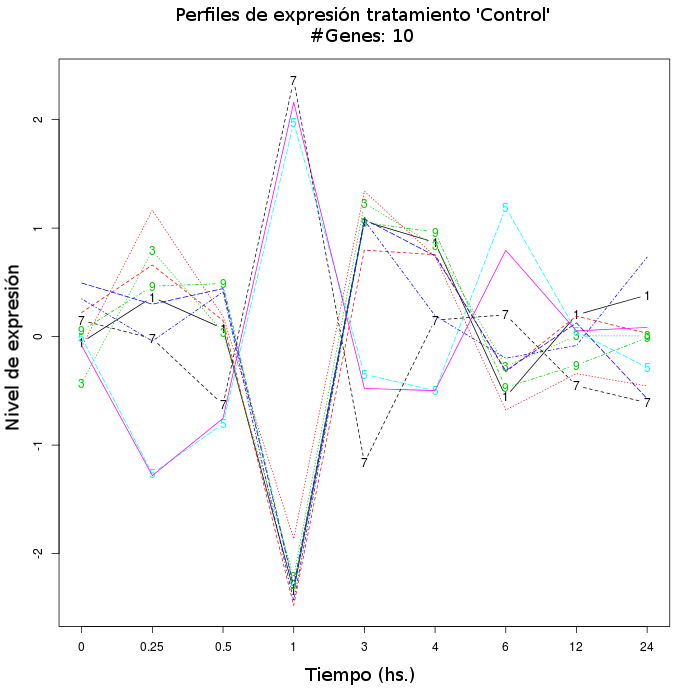
\includegraphics[width=1\textwidth]{perfiles_anti_coregulados}
    \caption{Perfiles de expresión para el tratamiento \textit{Control} de 10 genes que están co-regulados y anti co-regulados.}
    \label{fig:perfiles_anti_coregulados}
    \end{subfigure}
    \begin{subfigure}[t]{0.33\textwidth}
    \centering
    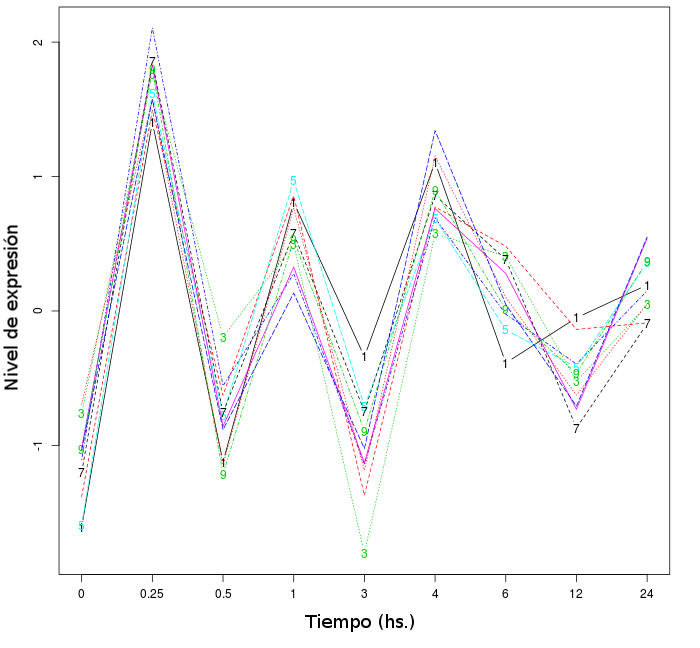
\includegraphics[width=1\textwidth]{perfiles_coregulados}
    \caption{Perfiles de expresión para el tratamiento \textit{Control} de 10 genes que están co-regulados.}
    \label{fig:perfiles_coregulados}
    \end{subfigure}
    \begin{subfigure}[t]{0.33\textwidth}
    \centering
    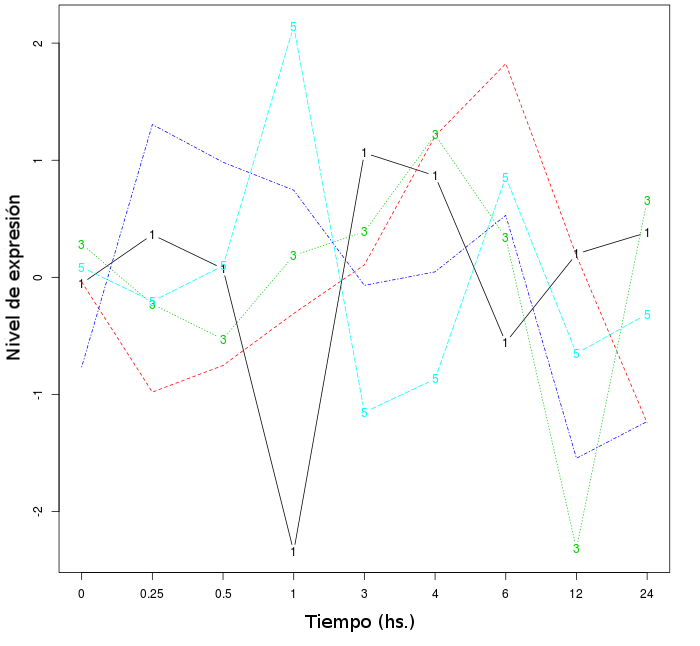
\includegraphics[width=1\textwidth]{perfiles_sin_agrupar}
    \caption{Perfiles de expresión para el tratamiento \textit{Control} de cinco genes tomados al azar.}
    \label{fig:perfiles_sin_agrupar}
    \end{subfigure}    
    \caption{Distintos grupos de perfiles de expresión}
\end{figure*}
Para dos puntos $\vec{x}$ e $\vec{y}$ en un espacio $d-dimensional$, representando el perfil de expresión de dos genes a lo largo de un dado tratamiento, el CCP se define como:
\begin{equation}
	r(\vec{x}, \vec{y}) = \frac{\sum\limits_{i=1}^d(x_i-\bar{x})(y_i-\bar{y})}{[\sum\limits_{i=1}^d(x_i-\bar{x})^2]^\frac{1}{2}[\sum\limits_{i=1}^d(y_i-\bar{y})^2]^\frac{1}{2}}
\end{equation}
El centrar alrededor de la media permite comparar la forma de ambos perfiles, en lugar de su magnitud.\\
El coeficiente de correlación $r$ varía entre $-1$ y $+1$. El caso $r = +1$, llamado \textit{correlación positiva perfecta}, ocurre cuando ambos genes tiene exactamente el mismo perfil, lo que se conoce como \hl{co-regulacion hacia arriba positiva (positive up-regulation) ver si este nombre esta bien}, mientras que el caso $r=-1$, llamado \textit{co-regulacion hacia abajo negativa perfecta}, ocurre cuando los perfiles son iguales pero opuestos. Un valor del CCP de $0$ implica que no se puede inferir una relación entre los perfiles de expresión.\\
La correspondiente medida de distancia puede ser calculada como \cite{Dhaeseleer2005}:
\begin{equation}
	d_{ccp}(\vec{x}, \vec{y}) = 1-r(\vec{x}, \vec{y})
	\label{eq:distancia_correlacion}
\end{equation}
o alternativamente:
\begin{equation}
	d_{ccp}(\vec{x}, \vec{y}) = 1-|r(\vec{x}, \vec{y})|
	\label{eq:distancia_correlacion_absoluta}
\end{equation}
En el caso de la distancia definida en \ref{eq:distancia_correlacion_absoluta}, al tomar el valor absoluto del CCP, genes cuyos perfiles son iguales pero opuestos (están anti co-regulados) pueden encontrarse más cerca en el sentido de $d_{ccp}$ que aquellos que son regulados hacia arriba o abajo pero en distintas magnitudes. Por lo tanto, esta distancia permite encontrar grupos de genes que son co-regulados, sin importar en que sentido (Figura \ref{fig:perfiles_anti_coregulados}) sean co-regulados.
En el caso de la distancia definida en \ref{eq:distancia_correlacion}, solamente se consideran cercanos aquellos genes cuyos perfiles sean co-regulados o bien hacia arriba o bien hacia abajo (Figura \ref{fig:perfiles_coregulados}).
\begin{figure}[h]

\end{figure}
\cite{Hennig2013}\cite{Kheng2010}\cite{Babu2004}\cite{Gan2007}\\
En el presente trabajo se utilizará como distancia la definida en \ref{eq:distancia_correlacion} para encontrar grupos de genes que únicamente se hayan co-regulado o bien hacia arriba o bien hacia abajo \cite{Eisen1998} \hl{discutir o buscar un paper mejor que justifique esto}.
\clearpage
\subsection{Similaridad semántica}
La adopción de ontologías provee los medios para comparar aspectos de entidades que de otra forma no podrían ser comparados. Por ejemplo, si dos productos génicos son anotados dentro del mismo esquema, es posible compararlos mediante la comparación de los términos en los cuales están anotados de forma explícita utilizando medidas de similaridad semántica. Se define una medida de similaridad semántica como una función tal que dados dos términos de la ontología o un conjunto de términos en los que dos genes están anotados, la función devuelve un escalar que refleja la cercanía de sentido entre ellos.\\
Es posible cuantificar la similaridad semántica en una ontología representada por un grafo como GO, mediante diversas estrategias.
\subsubsection{Comparación de términos en GO}
Existen esencialmente dos formas distintas de comparar términos en GO: comparación a partir de los arcos del grafo y comparación a partir de los nodos y sus propiedades. En este trabajo estaremos interesados únicamente en comparar términos a partir de sus nodos, ya que son los nodos los que contendrán la información biológica en forma de anotaciones génicas.\\
La comparación a partir de nodos se basa en comparar las propiedades de los términos involucrados, que pueden estar relacionadas con los términos en sí, sus ancestros o sus descendientes. 
Sea $C$ el conjunto de todos los términos de una ontología GO, con un número total $\#C$ de anotaciones. Un término $c_i$ tendrá $\#c_i$ anotaciones, ya sea directamente o por intermedio de cualquiera de sus hijos. La probabilidad de que un gen tomado al azar, sin otro tipo de información, se encuentre anotado al concepto $c_i$ será entonces $P(c_i) = \frac{\#c_i}{\#C}$, con $P:C\Rightarrow [0:1]$.\\
Se define el contenido de información de $c_i$ como $IC = -log_2(P(c_i))$, cantidad en el intervalo $(0, -log_2[\frac{1}{\#C}])$, que indica cuan específico e informativo es un término de la ontología. Para un $c_i$ y $c_j$ tales que $c_i \preceq c_j$, se tiene que $IC(c_i) \geq IC(C_j)$. Cuanto más específico sea un término, es menos probable que un gen dado esté anotado en el mismo, y por lo tanto, su contenido de información es mayor. El nodo raíz de la ontología tiene un contenido de información nulo, ya que es el ancestro de todos los términos de la misma y por lo tanto, saber que un concepto está anotado a la raíz no aporta información.\\
Si bien el IC puede tener un sesgo, ya que términos en áreas actuales de interés en investigaciones biomédicas van a estar más anotados que otros términos en otras áreas, la utilización del IC sigue teniendo un sentido desde el punto de vista de la probabilidad, porque es mucho más probable (y menos significativo) que dos genes compartan un término frecuentemente usado, que uno no tan frecuente, más allá de si ese término es frecuente porque sea genérico o porque sea un término de interés para la investigación actual.\\
Es posible definir una medida entre pares de términos utilizando el IC. El contenido de información puede ser aplicado a los ancestros en común que dos términos poseen, para cuantificar la información que comparten y medir entonces su similaridad semántica. Existen dos formas para ello: tomar el ancestro común más informativo (MICA, por sus siglas en inglés), en donde solo el ancestro común con mayor IC es considerado, o tomar el ancestro disjunto común (DCA por sus siglas en inglés), en la cual todos los ancestros comunes disjuntos (ancestros que no tienen ancestros comunes) son considerados.\\
Una de las medidas de similaridad semántica más comúnmente utilizadas es la medida de similaridad semántica introducida por Resnik en \cite{Resnik1995}, que consiste en asignar como la medida de similaridad entre dos términos, el contenido de información del primer ancestro en común (el MICA):
\begin{equation}
	Sim_{res}(c_i, c_j) = \max\limits_{c \in S(c_i, c_j)}(-log_2[P(c)]) = IC(MICA[c_i, c_j])
\end{equation}
Con $S(c_i, c_j)$ el conjunto de ancestros comunes de $c_i y c_j$.\\
A modo de ejemplo, tomemos el DAG de la figura \ref{fig:dag}, con 9 términos o conceptos: $C=\{R, c_0,...,c_7\}$ y con 5 entidades mapeadas (genes anotados): $g_1=\{5, 6, 2, 0, r\}$, $g_2=\{5, 4, 2, 3, 0, r\}$, $g_3=\{7, 1, r\}$, $g_4=\{4, 3, 0, r\}$ y $g_5=\{2, 0, r\}$. Podemos calcular la similaridad semántica de Resnik entre los términos $c_4$ y $c_5$, por ejemplo, sabiendo que $\#C = 5$ y que el ancestro común más informativo de ambos es $c_0$, con $\#c_0=4$. Se tiene entonces que $Sim_{res}(c_4, c_5) = IC(MICA) = IC(c_0) = -log_2(\frac{\#c_0}{\#C}) = -log_2(\frac{4}{5}) = 0.32$. Si quisieramos calcular ahora la similaridad semántica Resnik entre $c_5$ y $c_6$, obtendríamos $Sim_{res}(c_5, c_6) = IC(c_2) = -log_2(\frac{3}{5}) = 0.73$. Por lo tanto, para Resnik, los conceptos $c_5$ y $c_6$ son entre sí, más similares que los conceptos $c_4$ y $c_5$.\\
\begin{figure}[h]
    \centering
    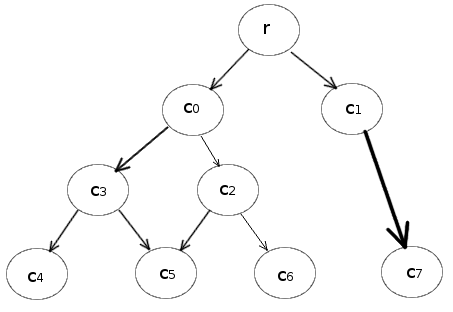
\includegraphics[width=0.5\textwidth]{dag}
    \caption{DAG con 9 términos o conceptos: $C=\{R, c_0,...,c_7\}$ y con 5 entidades mapeadas (genes anotados): $g_1=\{5, 6, 2, 0, r\}$, $g_2=\{5, 4, 2, 3, 0, r\}$, $g_3=\{7, 1, r\}$, $g_4=\{4, 3, 0, r\}$ y $g_5=\{2, 0, r\}$}
    \label{fig:dag}
\end{figure}
Al considerar solo el IC del MICA, la $Sim_{res}$ no tiene en cuenta la especificidad de los términos que compara, es decir, no toma en cuenta la distancia entre los términos y su MICA. Para tomar en cuenta esta distancia, las medidas de Lin \cite{Lin1998} y Jiang-Conrath \cite{Jiang1997} relacionan el IC del MICA con el IC de los términos a comparar:
\begin{equation}
	Sim_{lin}(c_i, c_j) = \frac{2\times IC(MICA[c_i, c_j])}{IC(c_i)+IC(c_j)}
\end{equation}
\begin{equation}
	Sim_{JC}(c_i, c_j) = 1-IC(c_i)+IC(c_j)-2\times IC(MICA[c_i, c_j])
\end{equation}Eisen1998
Un inconveniente de estas medidas es que se encuentran desplazadas del grafo, es decir, estas medidas son proporcionales a las diferencias entre los IC de los términos y de sus ancestros comunes, independientemente del valor absoluto de IC del ancestro.
Una restricción de todas estas medidas es que solo toman en cuenta el MICA, a pesar de que los términos GO pueden tener varios ancestros disjuntos comunes (DCA). Para evitar esta restricción, \cite{Pesquita2009} propuso la aproximación GraSM, que puede ser aplicada a todas las medidas descritas anteriormente, simplemente reemplazando el IC del MICA, por el promedio de los IC de los DCA. 
Existen más de dos docenas de medidas de similaridad entre términos GO, y no siempre es claro cuál es el mejor para un dado propósito. Sin embargo, generalmente la elección de una medida por defecto es suficiente\cite{Bose2016}. En este trabajo utilizaremos la $Sim_{res}$, por tratarse de una medida simple y efectiva.\\
Existen dos estrategias distintas para asignar una similaridad semántica entre genes. La primera se basa en medidas globales (groupwise en inglés), que comparan globalmente los conjuntos de términos en los que dos genes están anotados, $GO(g_1)$ y $GO(g_2)$, por ejemplo, contando cuantos términos comparten: $|GO(g_1) \cap GO(g_2)|$.\cite{Lee2004} \\
La segunda estrategia se basa en medidas de a pares (pairwise en inglés), calculando la similaridad semántica término a término de cada uno de los conjuntos $GO(g_1)$ y $GO(g_2)$ y luego aplicando sobre esta similaridad alguna operación para obtener una medida de similaridad entre estos genes.\\
El primer paso para esto es calcular una matriz de similaridad $S$ de $N\times M$ que contenga la similaridad de a pares, entre todos los pares de términos de estos conjuntos, con $N=|GO(g_1)|$ y $M=|GO(g_2)|$, utilizando alguna de las medidas de similaridad semántica entre términos presentadas anteriormente ($Sim_{res}$, $Sim_{lin}$, etc.):

\begin{equation}
	S_{ij} = Sim(GO(g_1^i), GO(g_2^j)), \forall i \in \{1,...,N\} y \forall j \in \{1,...,M\}
\end{equation}
Notar que esta matriz puede no ser simétrica.\\
Cada una de las $N$ filas corresponde a la similaridad entre la anotación $i-esima$ del gen $1$ y todas las $M$ anotaciones del gen $2$ y cada una de las $M$ columnas corresponde a la similaridad entre la anotación $j-esima$ del gen $2$ y todas las $N$ anotaciones del gen $1$.\\
A partir de $S_{ij}$ es posible definir tres métodos para obtener una medida de similaridad entre genes.
El primer método, propuesto en \cite{Sevilla2005}, consiste en tomar como similaridad, la máxima similaridad entre todos los términos:
\begin{equation}
	Sim_{max}(GO(g_i), GO(g_j)) = \max\{S_{ij}\}
\end{equation}
El segúndo método, propuesto en \cite{Lord2003}, consiste en tomar el valor medio de todos los valores de la matriz $S_{ij}$:
\begin{equation}
	Sim_{med}(GO(g_i), GO(g_j)) = \frac{1}{N.M}\sum\limits_{i,j}S_{ij}
\end{equation}
Finalmente, el tercer método, propuesto en \cite{Pesquita2009}, implica tomar el valor medio de los máximos de cada fila, el valor medio de los máximos de cada columna, y quedarse con el máximo de esos dos valores. Este criterio de similaridad se conoce como \textit{rcmax}:
\begin{equation}
	Sim_{rcmax}(GO(g_1), GO(g_2)) = \max\{\frac{1}{N}\sum\limits_{i}\max\limits_{1\leq j \leq M}S_{ij}, \frac{1}{M}\sum\limits_{j}\max\limits_{1\leq i \leq N}S_{ij}\}
\end{equation}
Como muchos genes están anotados en conceptos muy diversos por participar en procesos biológicos muy distintos, e incluso puede haber genes que no están anotados en ningún concepto, la medida de similaridad $Sim_{med}$ tiende a dar valores más bajos que otros métodos. Por el contrario, la medida $Sim_{max}$ tiende a dar valores más altos, por ser una medida más optimista. En este trabajo utilizaremos el tercer método, $Sim_{rcmax}$, por ser un compromiso entre ambos casos extremos.
\cite{Resnik1995}\cite{Pesquita2009}\cite{Bose2016}\cite{Lin1998}\cite{Jiang1997}\cite{Sevilla2005}\cite{Lord2003}

\section{Estrategias de agrupamiento}
En lo que sigue introduciremos las diferentes estrategias de agrupamiento de datos utilizadas en este trabajo, tanto para agrupamiento de perfiles transcripcionales como de armado de comunidades en las redes presentadas anteriormente.\\
Es posible distinguir dos tipos de agrupamientos, conocidos como agrupamiento duro (hard clustering en inglés), y agrupamiento difuso (fuzzy clustering en inglés). En el primer caso, el de agrupamiento duro, cada objeto del conjunto de datos es asignado a un y solo un grupo, mientras que en el segundo caso, el de agrupamiento difuso, un elemento del conjunto puede pertenecer a varios grupos, con distinta probabilidad. En este trabajo utilizaremos únicamente métodos de agrupamiento duro.\\
\section{Agrupamientos no jerárquicos}
Además la distinción mencionada más arriba, los métodos de agrupamiento pueden dividirse (entre otros) fundamentalmente entre agrupamientos jerárquicos y agrupamientos no jerárquicos.
Las dos estrategias de agrupamientos no jerárquicos que se presentan a continuación fueron utilizadas en el desarrollo de este trabajo.
\subsection{K-means}
K-means es un método usual de agrupamiento no jerárquico en donde cada observación pertenece al grupo con la media más cercana a la observación.\\
El mismo comienza agrupando los objetos de forma arbitraria en $K$ grupos distintos. El número $K$ puede ser elegido de forma aleatoria o estimado mediante algún otro método de agrupamiento jerárquico pero es siempre fijo. Luego, se calcula un promedio de la posición de todas las observaciones de cada grupo, llamado centroide. A continuación, los objetos individuales son redistribuidos de un grupo a otro dependiendo de que centroide esté más cerca de la observación. Este procedimiento de calcular el centroide de cada cluster y re agrupar los objetos más cercanos a los centroides disponibles se repite de manera iterativa una cantidad fija de veces o hasta la convergencia del método (se considera que el método converge cuando una iteración no modifica la iteración anterior).\\
Típicamente, se requieren entre 20000 y 100000 iteraciones para la convergencia del método, aunque no hay garantías de que eso ocurra.
Más formalmente, sea un conjunto de observaciones $\{\vec{x_1},...,\vec{x_n}\}$, k-means construye una partición de las observaciones en $k$ grupos con $k \leq n$ a fin de minimizar una función de costo, como ser la suma de los cuadrados dentro de cada grupo $G = \{g_1,...,g_k\}$: 
\begin{equation}
	C = argmin\sum\limits_{i=1}^k \sum\limits_{x_j \in g_i}||x_j-\mu_i||
\end{equation}
Con $\mu_i$ el valor medio de los elementos del grupo $g_i$.
La figura \ref{fig:ejemplo_k_means} muestra un conjunto de observaciones y los grupos que se obtienen fijando $k=2$ y $k=5$, junto con sus respectivos centroides.
\begin{figure}[h]
    \centering
    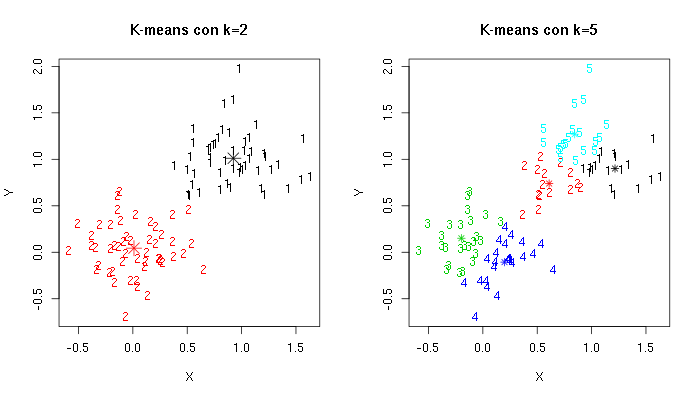
\includegraphics[width=0.8\textwidth]{ejemplo_k_means}
    \caption{Agrupamiento utilizando k-means con $k=2$ y $k=5$. \hl{mejorar epigrafe}}
    \label{fig:ejemplo_k_means}
\end{figure}
Se observa que dependiendo del $k$ utilizado, el algoritmo encuentra particiones con mayor o menor nivel de \textit{resolución}. Volveremos sobre el tema de la resolución más adelante.
\cite{Kogan2006}\cite{Hartigan1979}

\subsection{PAM}
Si bien k-means es uno de los métodos de partición más utilizados ya que es muy eficiente en términos de tiempo computacional, el mismo es muy sensible a observaciones aisladas. Por esta razón, en algunos métodos se reemplazan los centroides, que son puntos no necesariamente pertenecientes al conjunto de observaciones, por medoides, que son los objetos más centrales dentro del grupo (se reemplaza k-means por k-medoids). Esto hace que el método sea insensible a observaciones aisladas.\\
Particionar alrededor de medoides (Partitioning around medoids en inglés) es uno de los métodos más conocidos que hace uso de este concepto, buscando minimizar la función de costo:
\begin{equation}
	C = argmin\sum\limits_{i=1}^k \sum\limits_{x_j \in g_i} d(x_j, m_i)
\end{equation}
Con $m_i$ el medoide del grupo $i$ y $d(x_j, m_i)$ la distancia entre el objeto $x_j$ del grupo $i$ y el medoide del mismo grupo.
\cite{Park2009}\cite{Ibrahim2012}
\section{Agrupamientos jerárquicos}
Existen dos acercamientos distintos para realizar un agrupamiento jerárquico: se puede ir ``desde abajo hacía arriba'', agrupando grupos más chicos en grupos más grandes, lo que se conoce como agrupamiento aglomerativo, ose puede ir ``desde arriba hacia abajo'', dividiendo grupos más grandes en grupos más chicos, lo que se conoce como agrupamiento divisivo. En este trabajo nos interesará únicamente trabajar con agrupamientos aglomerativos.\\
Un agrupamiento jerárquico aglomerativo comienza con cada objeto en un grupo separado. Luego, se unen los dos grupos más cercanos de acuerdo a algún criterio definido generando un nuevo grupo a partir de ambos. Al nuevo grupo se le asignará una distancia al resto de los grupos de acuerdo a cierto criterio. Esto se repite hasta que solo quede un único grupo.\\
Es un tipo de procedimiento determinista y voraz (greedy en inglés), ya que realiza las decisiones tomando en cuenta los óptimos locales en cada etapa, esperando obtener con esto un óptimo global.\\
Se dice que una partición es más fina (o un refinamiento) de otra partición, si cada grupo de una partición más fina está contenido dentro de un grupo de la partición más gruesa, es decir, cada grupo de la partición más fina es un sub-grupo de un grupo de la partición más gruesa. El agrupamiento jerárquico es un método cuyo resultado es un conjunto de particiones anidadas $P_n, P_{n-1}, ..., P_1$ cada vez más gruesas, donde cada nivel más alto une dos grupos de una partición de un nivel más bajo.\\
Para poder realizar este procedimiento, es necesario definir cuan cercanos son dos grupos:
\subsection{Método de Ward}
Este método busca unir los grupos de una forma tal que se minimice la pérdida de información asociada a cada unión, usualmente cuantificada como el error de la suma de los cuadrados (ESS). Dado un conjunto de puntos $C$, el ESS asociado a $C$ queda definido por:
\begin{equation}
	ESS(C) = \sum\limits_{\vec{x} \in C}(\vec{x}-\mu (C))(\vec{x}-\mu (C))^T
\end{equation}
con $\mu (C) = \frac{1}{|C|}\sum\limits_{\vec{x} \in C}\vec{x}$, el valor medio de $C$. Suponiendo que una dada partición está separada en $k$ grupos, $\{C_1, C_2,...,C_k\}$, entonces se tiene que la pérdida de información de la partición está dada por:
\begin{equation}
	ESS = \sum\limits_{i=1}^k ESS(C_i)
	\label{eq:ESS}
\end{equation}
En cada etapa de este método, se prueban todas las uniones de grupos posibles de a pares y se realiza aquella unión que minimiza \ref{eq:ESS}.\\
En el agrupamiento jerárquico, el ESS comienza en cero, ya que cada punto pertenece a un grupo distinto, y crece a medida que se unen grupos. Al ser un algoritmo voraz, la ESS para un dado número de grupos $k$ no será necesariamente la mínima.
\subsection{Método de enlace único (o single-link en inglés)}
Este método es uno de los métodos más simples para agrupamiento jerárquico. El mismo define la distancia entre dos grupos como la mínima distancia entre entre sus miembros. Sean $C_i$ y $C_j$ dos grupos, entonces la distancia de enlace único se define como:
\begin{equation}
	D_{sl}(C_i, C_j) = \min\limits_{\vec{x} \in C_i, \vec{y} \in C_j} d(\vec{x}, \vec{y})
\end{equation}
con $d(\vec{x}, \vec{y})$ la función de distancia utilizada para calcular la matriz de disimilaridad entre los elementos.
El nombre de enlace único hace referencia a que dos grupos están cerca aunque tengan un único par de puntos cerca. Este método permite el manejo de grupos con formas complejas y es invariante ante transformaciones monótonas (como una transformación logarítmica) \cite{Johnson1967}.\\
Este algoritmo solamente considera la separación entre elementos, dejando de lado la compacidad o el balance en los grupos.
\subsection{Método de enlace completo (o complete-link en inglés)}
Este método es similar al método de enlace único, ya que toma la distancia entre dos grupos como el máximo de la distancia entre sus puntos:
\begin{equation}
	D_{cl}(C_i, C_j) = \max\limits_{\vec{x} \in C_i, \vec{y} \in C_j} d(\vec{x}, \vec{y})
\end{equation}
con $d(\vec{x}, \vec{y})$ la función de distancia utilizada para calcular la matriz de disimilaridad entre los elementos.\\
En este trabajo, utilizaremos el método de enlace completo.
\cite{Shalizi2009}\cite{Gan2007}\cite{Johnson1967}

\subsection{Representación de un agrupamiento jerárquico - dendrogramas}
Un agrupamiento jerárquico puede representarse como un árbol, llamado dendrograma, que permite una rápida interpretación. En un dendrograma, cada nodo está asociado con una altura $h$, tal que si $A$ y $B$ son dos nodos del dendrograma, $h$ cumple:
\begin{equation}
	h(A) \leq h(B) \Leftrightarrow A \subseteq B
\end{equation}
A modo ilustrativo, la figura \ref{fig:agrupamiento_jerarquico} muestra el agrupamiento jerárquico realizado sobre 10 puntos colocados de forma aleatoria en el plano, agrupados utilizando la distancia euclidiana y mediante los tres métodos vistos anteriormente (Ward, enlace único y enlace completo).
\begin{figure}[h]
    \centering
    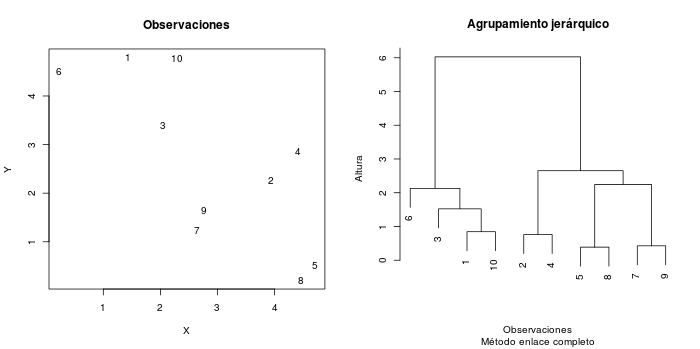
\includegraphics[width=0.8\textwidth]{agrupamiento_jerarquico}
    \caption{Ejemplos de agrupamientos jerárquicos utilizando el mismo conjunto de datos pero distintos métodos de distancia entre grupos.\hl{mejorar epigrafe}}
    \label{fig:agrupamiento_jerarquico}
\end{figure}
De estos gráficos es claro que cada método produce una secuencia diferente de particiones, y dependerá de la aplicación que se requiera, cual de los métodos utilizar.
\section{Detectando grupos en el agrupamiento jerárquico}
El agrupamiento jerárquico organiza los objetos en árboles (dendrogramas) cuyas ramas son los grupos deseados. El proceso de detección de grupos se conoce como corte de árbol, corte de ramas o podado de ramas. 
\subsection{Corte de árbol estático}
El método más sencillo de podado es conocido como corte de árbol estático, y funciona definiendo cada rama contigua debajo de una altura fija de corte, como un grupo separado. La cantidad de grupos obtenidos por éste método depende fuertemente de la altura de  corte elegida. La figura \ref{fig:corte_arbol_estatico} muestra dos alturas de corte posibles y los grupos que se obtienen a partir de cada una de ellas.
\begin{figure}[h]
    \centering
    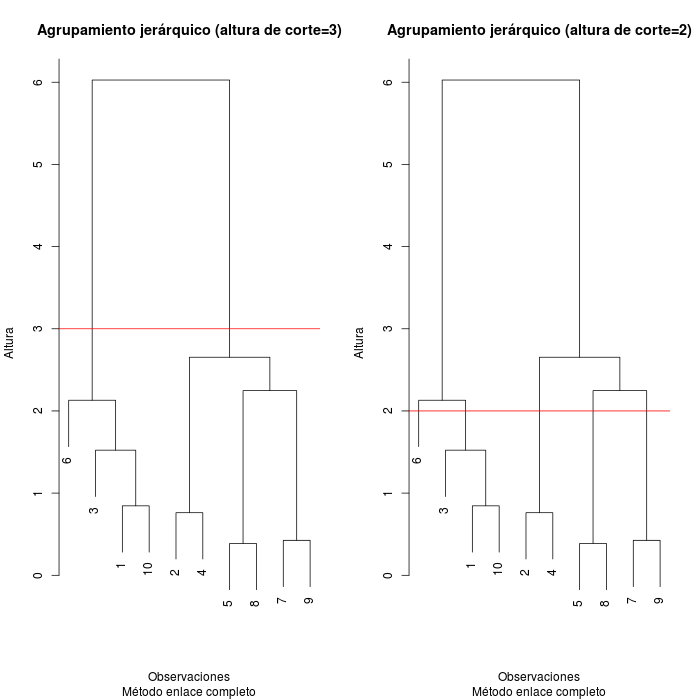
\includegraphics[width=0.8\textwidth]{corte_arbol_estatico}
    \caption{Corte de árbol a dos alturas diferentes. \hl{mejorar epigrafe}}
    \label{fig:corte_arbol_estatico}
\end{figure}
Al cortar el árbol en $h=3$, se obtienen dos grupos, el grupo $g_1$, que contiene a las observaciones $\{6, 3, 1, 10\}$ y el grupo $g_2$ que contiene a las observaciones $\{2, 4, 8, 5, 7, 9\}$, mientras que al cortarlo en $h=2$, se obtienen cuatro grupos, $g_1'$ con la observación $\{6\}$, $g_2'$ con las observaciones $\{3, 1, 10\}$, $g_3'$ con las observaciones $\{2, 4\}$ y $g_4'$ con las observaciones $\{5, 8, 7, 9\}$.\\
A partir de un ejemplo tan sencillo es inmediato notar que el problema del agrupamiento es un problema ``mal planteado'', es decir, cualquier conjunto de puntos puede ser agrupado de maneras drásticamente distintas, sin que exista actualmente un criterio para preferir uno u otro agrupamiento. La fuente de ambigüedades a este respecto más importante, es que la forma en que los datos deberían ser agrupados, depende fuertemente de la \textit{resolución} deseada. Lo que parece una única nube de puntos puede resultar ser, al analizar los datos con mayor resolución, una partición compuesta de muchos grupos. Cada taréa deberá encontrar el nivel adecuado de resolución para obtener la cantidad ``correcta'' de grupos.\cite{Domany1999}\cite{Langfelder2008}
\subsection{Corte de árbol dinámico híbrido}
Si bien es posible detectar grupos distintos en el dendrograma a partir de una inspección visual, utilizar una técnica de corte de árbol estático de forma programática no siempre logra identificar adecuadamente los grupos. Este no es un inconveniente del método de agrupamiento jerárquico, sino que al poseer grupos anidados, un solo corte a una altura prefijada no será capaz de detectarlos todos. El método de corte de árbol dinámico híbrido ataca este problema analizando la forma de las ramas del dendrograma en lugar de una altura absoluta. El mismo construye los grupos de abajo hacia arriba en dos pasos. En el primer paso, se detectan las ramas que satisfacen un criterio específico para ser grupos. Este paso de poda está basado en la información de unión del dendrograma. En el segundo paso, se miden cuán cerca de los grupos detectados en el primer paso están todos los objetos no asignados previamente. Si un objeto está suficientemente cerca de un grupo, es asignado a ese grupo. En este paso, se ignora el dendrograma y se utiliza únicamente la información de disimilaridad. Este paso puede considerarse un método modificado de particionado alrededor de medoides (modified Partitioning Around Medoids o mPAM, en inglés). Por eso el nombre de \textit{híbrido}, al tratarse de una mezcla entre agrupamiento jerárquico y no jerárquico.
Los criterios específicos para la detección de grupos se basan en los siguientes cuatro criterios de la forma de las ramas:
\begin{enumerate}
\item Un grupo debe tener una cantidad mínima de objetos.
\item Los objetos que están muy lejos del grupo son excluidos del grupo aunque pertenezcan a la misma rama del dendrograma.
\item Cada grupo debe estar separado de su entorno por una brecha o espacio vacío.
\item El núcleo de cada grupo (el conjunto de objetos con menor altura de unión en el grupo) debe estar fuertemente conectado.
\end{enumerate}
O más formalmente, dado un núcleo de un grupo, llamamos $d$ al promedio de las disimilaridades de a pares entre objetos del núcleo, es decir, a su dispersión y definimos la brecha $g$ de un grupo como la diferencia entre $d$ y la altura donde el grupo se une al resto del dendrograma y entonces, una rama se considera un grupo si:
\begin{enumerate}
\item Tiene al menos $N_0$ objetos.
\item Todas las alturas de unión son a lo sumo de $h_{max}$.
\item La brecha $g$ del grupo es mayor que un $g_{min}$.
\item La dispersión $d$ del núcleo es a lo sumo $d_{max}$.
\end{enumerate}
Los parámetros $N_0$, $h_{max}$, $g_{min}$ y $d_{max}$ son parámetros ajustables del método.
\begin{figure}[h]
    \centering
    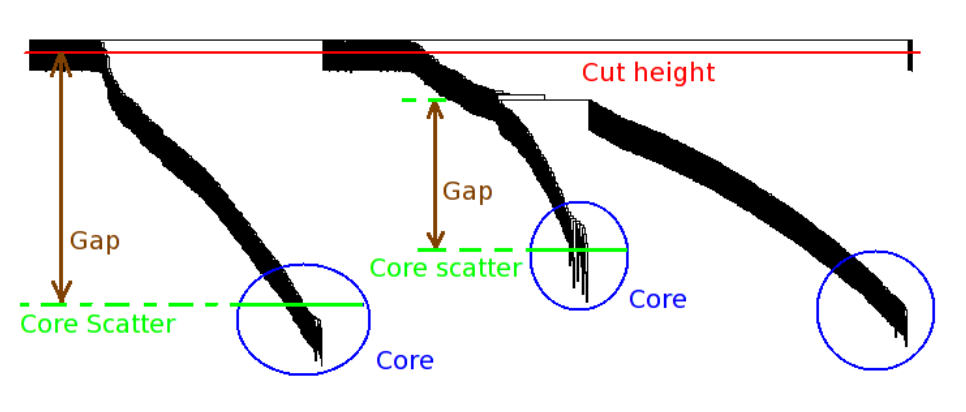
\includegraphics[width=0.8\textwidth]{cut_tree_dynamic_ejemplo}
    \caption{Dendrograma simulado con tres ramas con alturas de unión diferentes. La altura de corte corresponde a $h_{max}$. \hl{poner en castellano y citar correctamente}}
    \label{fig:cut_tree_dynamic_ejemplo}
\end{figure}
La figura \ref{fig:cut_tree_dynamic_ejemplo} muestra un ejemplo de los parámetros utilizados para definir los grupos en el paso 1.\\
Para el paso 2, de tipo PAM, los objetos no asignados (o aquellos grupos que no cumplan tener al menos $N_0$ objetos) son asignados al grupo más cercano si la disimilaridad correspondiente es más pequeña que una disimilaridad máxima definida previamente, o si es más pequeña que el ``radio'' del grupo. El ``radio'' se define como la máxima de las disimilaridades del medoide del grupo al resto de los objetos del mismo.\\
Es posible controlar la sensibilidad de las divisiones de los grupos mediante el parámetro \textit{deepSplit}, que puede tomar los valores de 1 a 4. Para un $deepSplit=1$, el método producirá relativamente pocos grupos, de muchos elementos y bien definidos, mientras que para $deepSplit=4$, el método producirá más grupos pero con una dispersión mayor en el núcleo y separado por brechas más pequeñas.\\
Para una descripción más detallada del algoritmo, el lector interesado puede referirse a \cite{Langfelder2008}, \cite{Langfelder2007}.
\section{Infomap y CNM}
Como se desarrolló en la sección \ref{sec:redes}, las redes son construcciones útiles para esquematizar la organización de las interacciones en distintos tipos de sistemas. Sin embargo, por motivos de visualización, solo se pueden representar pequeños sistemas. Las redes reales son usualmente tan grandes que es necesario representarlas mediante algún mecanismo de granularidad más gruesa, es decir, descomponer a la red en módulos que representen varios nodos y arcos. Este es el objetivo básico de lo que se conoce como \textit{detección de comunidades}.\\
En este trabajo utilizaremos dos métodos de modularización en redes, Infomap y CNM.\\
El método o algoritmo Infomap hace uso de criterios de optimización basados en teorías de información, donde los módulos se definen de tal forma que la longitud media de la descripción de un proceso de paseo al azar en el grafo sea mínima, mientras que el algoritmo de Clauset-Newman-Moore (CNM), a partir de ciertas heurísticas, busca particiones de la red optimizando directamente una función de calidad $Q$.\\
Ambos métodos serán utilizados en este trabajo con el fin de comparar los resultados obtenidos para las comunidades Infomap y CNM con los obtenidos para los métodos de agrupamiento usados.\cite{Berenstein2014}\cite{Rosvall2008}\\
Distintos métodos darán distintos resultados, dependiendo del conjunto de datos y del objetivo del agrupamiento, por lo que es de vital importancia elegir el método adecuado a la aplicación en cuestión. Las figuras \ref{fig:ejemplo_k_means_ward_single} y \ref{fig:ejemplo_k_means_ward_single_2} muestran ejemplos de conjuntos de datos diversos y de como son agrupados por los distintos métodos.
\begin{figure}[h]
    \centering
    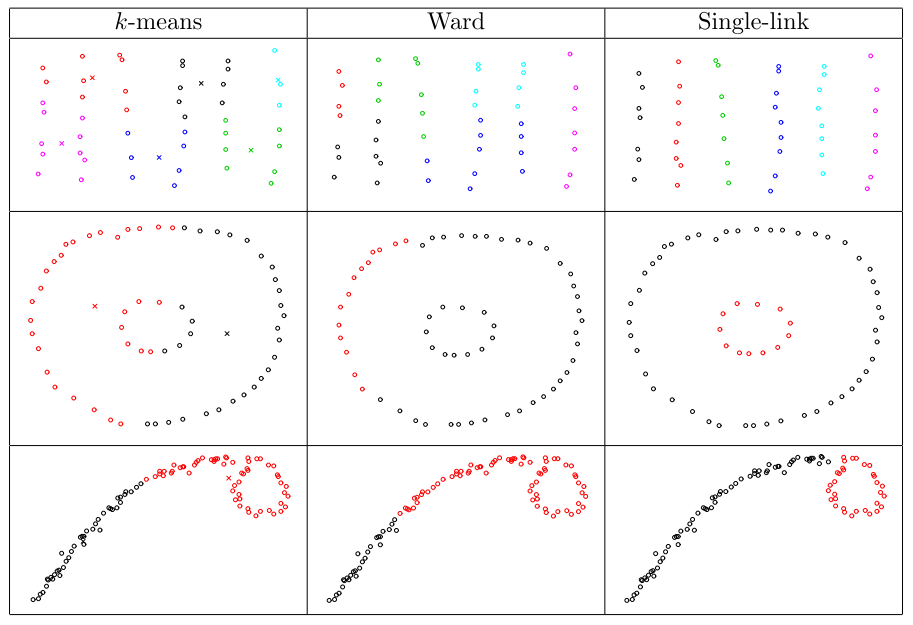
\includegraphics[width=0.8\textwidth]{ejemplo_k_means_ward_single}
    \caption{Algunos casos para los cuales el método de enlace único (single-link) se comporta ``mejor'' que los métodos de k-means o de Ward .\hl{citar correctamente}}
    \label{fig:ejemplo_k_means_ward_single}
\end{figure}

\begin{figure}[h]
    \centering
    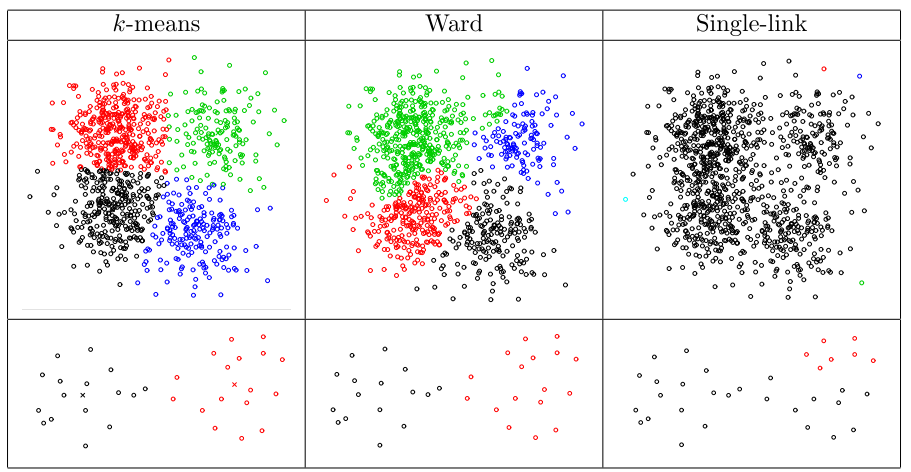
\includegraphics[width=0.8\textwidth]{ejemplo_k_means_ward_single_2}
    \caption{Algunos casos para los cuales los métodos de k-means o de Ward se comportan ``mejor'' que el método de enlace único (single-link).\hl{citar correctamente}}
    \label{fig:ejemplo_k_means_ward_single_2}
\end{figure}

\subsection{Matriz de similaridad topológica - TOM y GTOM}
\hl{completar con tom y gtom}